\section{Problem 2}~\label{sec:prob2}

\subsection{} % 2.1

\begin{equation}
    f_{11}(x_1) = \begin{cases}
            -1, \quad \text{when }x_1\le 0.5, \\
            1, \quad\quad \text{otherwise}.
        \end{cases}
\end{equation}
\begin{equation}
    f_{12}(x_2) = \begin{cases}
            -1, \quad \text{when }x_2\le 0.5, \\
            1, \quad\quad \text{otherwise}.
        \end{cases}
\end{equation}
\begin{equation}
    g(h_{11}, h_{12}) = h_{11} h_{12}.
\end{equation}

\subsection{} % 2.2

\begin{figure}[ht]
\begin{minipage}[b]{0.45\linewidth}
\centering
    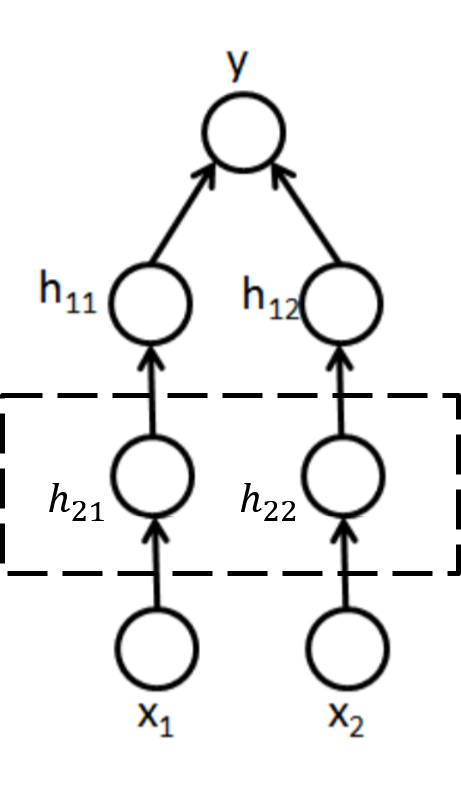
\includegraphics[width=0.5\linewidth]{fig/insert.png}
    \caption{\small
    new layer.}
    \label{fig:insert}
\end{minipage}
\hspace{0.5cm}
\begin{minipage}[b]{0.45\linewidth}
\centering
    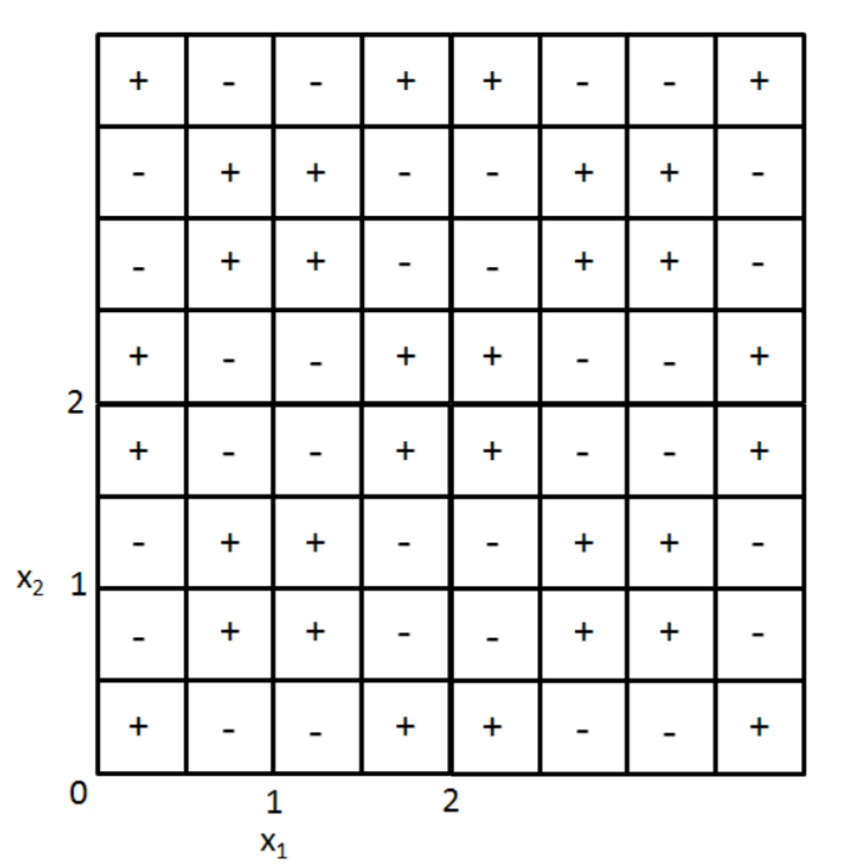
\includegraphics[width=0.8\linewidth]{fig/4x4.png}
    \caption{\small
    $4\times 4$ pattern.}
    \label{fig:4x4}
\end{minipage}
\end{figure}

Like in Figure~\ref{fig:insert},
we insert a layer above the input,
which contains two neurons
$h_{21}=f_{21}(x_1)$,
$h_{22}=f_{22}(x_2)$, and

\begin{equation}
    f_{21}(x_1) = \begin{cases}
            x_1, \quad\quad\quad \text{when }x_1\le 1, \\
            2-x_1, \quad \text{otherwise}.
        \end{cases}
\end{equation}
\begin{equation}
    f_{22}(x_2) := f_{21}(x_2).
\end{equation}

\subsection{} % 2.3

Image the input region as a piece of paper in squared shape.
Fold them horizontally and vertically along the center line,
we will reduce a $2\times 2$ square to a $1\times 1$ square.
Folding like this multiple times will be able to create more
complex patterns.
So such regularity and global structure is a complex symmetry pattern
that resulted from this folding process.
An example of $4\times 4$ square is shown if Figure~\ref{fig:4x4}.

\subsection{} % 2.4
